\section{Proposta}

\subsection{Proposta}

\begin{frame}\frametitle{Proposta}
\begin{itemize}
	\item O objetivo deste trabalho � construir um arcabou�o para a cria��o de terrenos proceduralmente em tempo real e que permita a inser��o de modelos pelo usu�rio, como, por exemplo, na forma de mapas de altura.
	\item �reas gen�ricas ser�o geradas proceduralmente, e �reas que necessitam de maior detalhe, ser�o visualizadas por meio de mapas de altura.
\end{itemize}
\end{frame}

\begin{frame}\frametitle{Proposta}
\begin{itemize}
	\item O arcabou�o est� sendo constru�do de forma que possa suportar terrenos criados de diversas maneiras.
	\begin{itemize}
		\item Arquivos com mapas de altura
		\item Fault Formation
		\item Perlin Noise (Ru�do de Perlin)
		\item Fbm
	\end{itemize}
\end{itemize}
\begin{center}
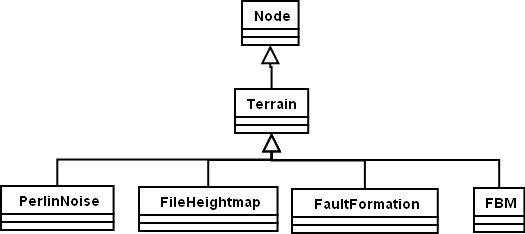
\includegraphics[width=0.5\linewidth]{img/node}
\end{center}
\end{frame}

\subsection{Gera��o procedural dos terrenos}

\begin{frame}\frametitle{Ru�do de Perlin}
\begin{columns}
	\begin{column}{5cm}
	\begin{itemize}
		\item O ru�do � usado para simular estruturas naturais, como n�vens, texturas de �rvores, e terrenos.
	\end{itemize}
	\vspace{3cm} 
	\end{column}
	\begin{column}{5cm}
	\begin{overprint}
		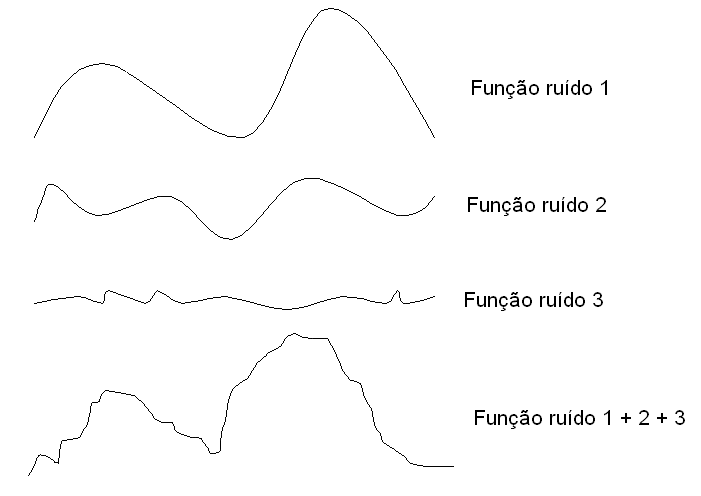
\includegraphics[width=1.0\linewidth]{img/perlin}
	\end{overprint}
	\end{column}
\end{columns}
\end{frame}


\subsection{Grafo de cena}

\begin{frame}\frametitle{Grafo de cena - Organiza��o}
\begin{columns}
	\begin{column}{5cm}
	\begin{itemize}
		\item Um grafo para armazenar os terrenos que ser�o renderizados.
		\item Um nodo do grafo de cena aponta para os oito terrenos vizinhos.
		\item Quando a c�mera muda de terreno, novos terrenos s�o gerados.
		\item Os v�rtices s�o armazenados em uma estrutura de dados VBO.
	\end{itemize}
	\vspace{3cm} 
	\end{column}
	\begin{column}{5cm}
	\begin{overprint}
		\includegraphics<1>[width=1.0\linewidth]{img/grafo_cena2}
		\includegraphics<2>[width=1.0\linewidth]{img/grafo_cena3}
	\end{overprint}
	\end{column}
\end{columns}
\end{frame}


